\begin{itemize}
\item[(a)]

\begin{figure}[h]
    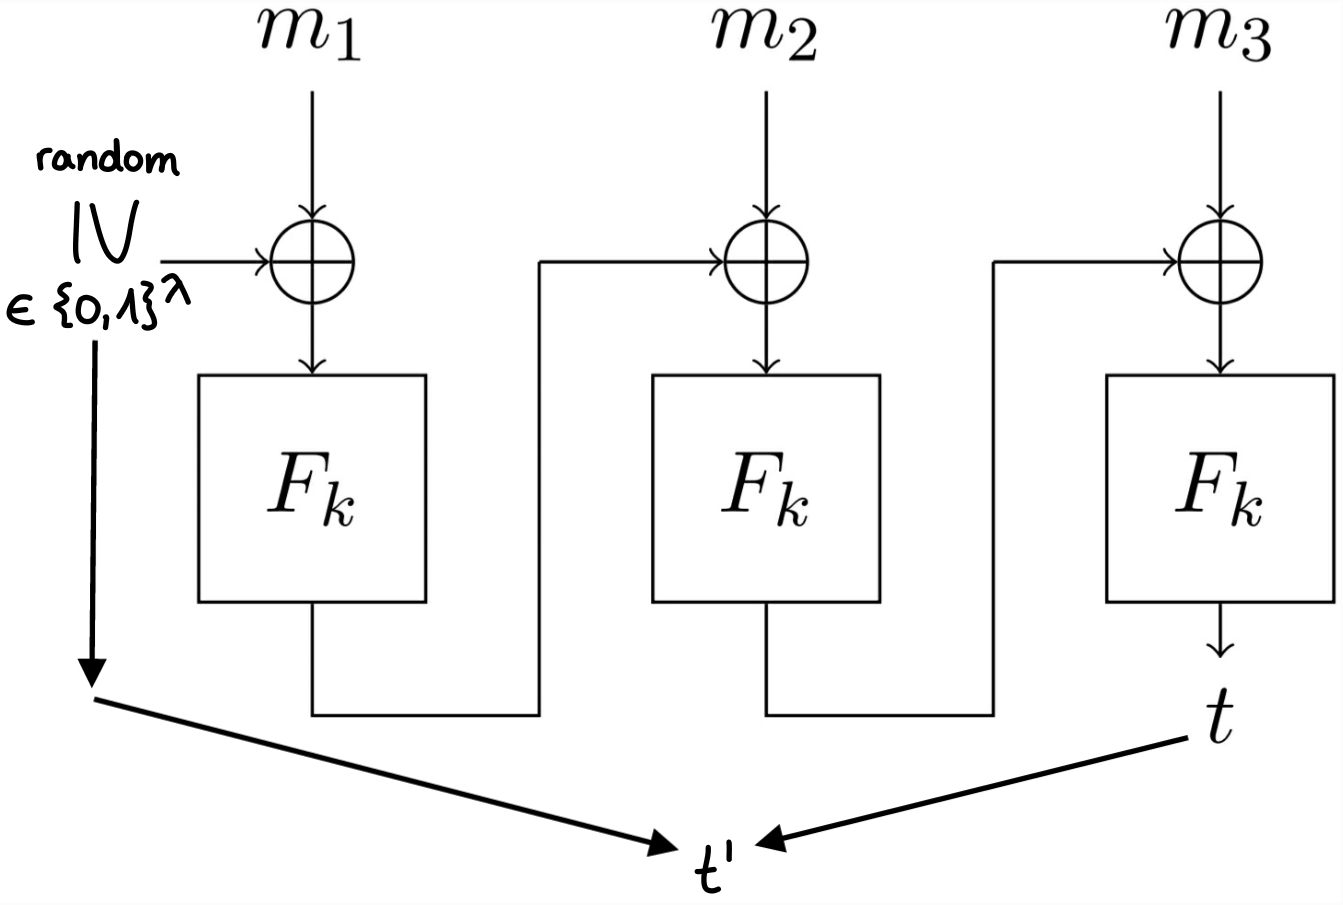
\includegraphics[width=\textwidth,height=\textheight,keepaspectratio]{ModKrypt_7-3a.jpg}
    \centering
\end{figure}


The adversary \(\mathcal{A}\) can choose the message m\(^{*}\) of length \(\ell\)(\(\lambda\)) \(\cdot\) \(\lambda\). We set \(\ell\)(\(\lambda\)) = l \\
m\(^{*}\) =  m\(_{1}^{*}\) \(\vert \vert\) ...  \(\vert \vert\)  m\(_{l}^{*}\). We set m\(_{i}^{*}\) =  0\(^{\lambda}\). \\
We query m\(^{*}\) to our Mac\(_{k}\)(\(\cdot\)) oracle and recieve the tag t´\(^{*}\) = (IV\(^{*}\), t\(^{*}\)). IV\(^{*}\) \(\in\) \(\{\)0,1\(\}\)\(^{\lambda}\) is a randomly generated vector.\\
\\
c\(_{1}^{*}\) = F\(_{k}\)(IV\(^{*}\) \(\xor\) m\(_{1}^{*}\)) =  F\(_{k}\)(IV\(^{*}\) \(\xor\) 0\(^{\lambda}\)) = F\(_{k}\)(IV\(^{*}\)) \\
c\(_{2}^{*}\) = F\(_{k}\)(c\(_{1}^{*}\) \(\xor\) m\(_{2}^{*}\)) =  F\(_{k}\)(F\(_{k}\)(IV\(^{*}\)) \(\xor\) 0\(^{\lambda}\)) = F\(_{k}\)( F\(_{k}\)(IV\(^{*}\))) \\
... \\
c\(_{l}^{*}\) = F\(_{k}\)( ... F\(_{k}\)(IV\(^{*}\)) ...) = t\(^{*}\) \\
\\
To break the security of the MAC the adversary \(\mathcal{A}\) can construct the following forgery: \\
m = 0\(^{\lambda-1}\)1 \(\vert \vert\) m\(_{2}^{*}\) \(\vert \vert\) ...  \(\vert \vert\)  m\(_{l}^{*}\)
with IV = IV\(^{*}\) \(\xor\) 0\(^{\lambda-1}\)1 \\
meaning we flip the last bit of the first block of our message as well as the last bit of our IV\(^{*}\).\\
This causes that IV\(^{*}\) \(\xor\) m\(_{1}^{*}\) = IV \(\xor\) m\(_{1}\) and therefore \\ c\(_{1}^{*}\) = F\(_{k}\)(IV\(^{*}\) \(\xor\) m\(_{1}^{*}\)) =  F\(_{k}\)(IV \(\xor\) m\(_{1}\)) = c\(_{1}\) as well as all other c\(_{i}^{*}\) = c\(_{i}\) of the chain for i \(\in\) \(\{\)2,l\(\}\).\\
\\
We can conclude that t\(^{*}\) = t but m\(^{*}\) \(\neq\) m and therefore m was not queried to Mac\(_{k}\) before. \\
\(\Rightarrow\) The adversary \(\mathcal{A}\) can now create the valid forgery (m, t´) with t´ = (IV, t\(^{*}\)) and can break the unforgability of the Mac.

\item[(b)]

\begin{figure}[h]
    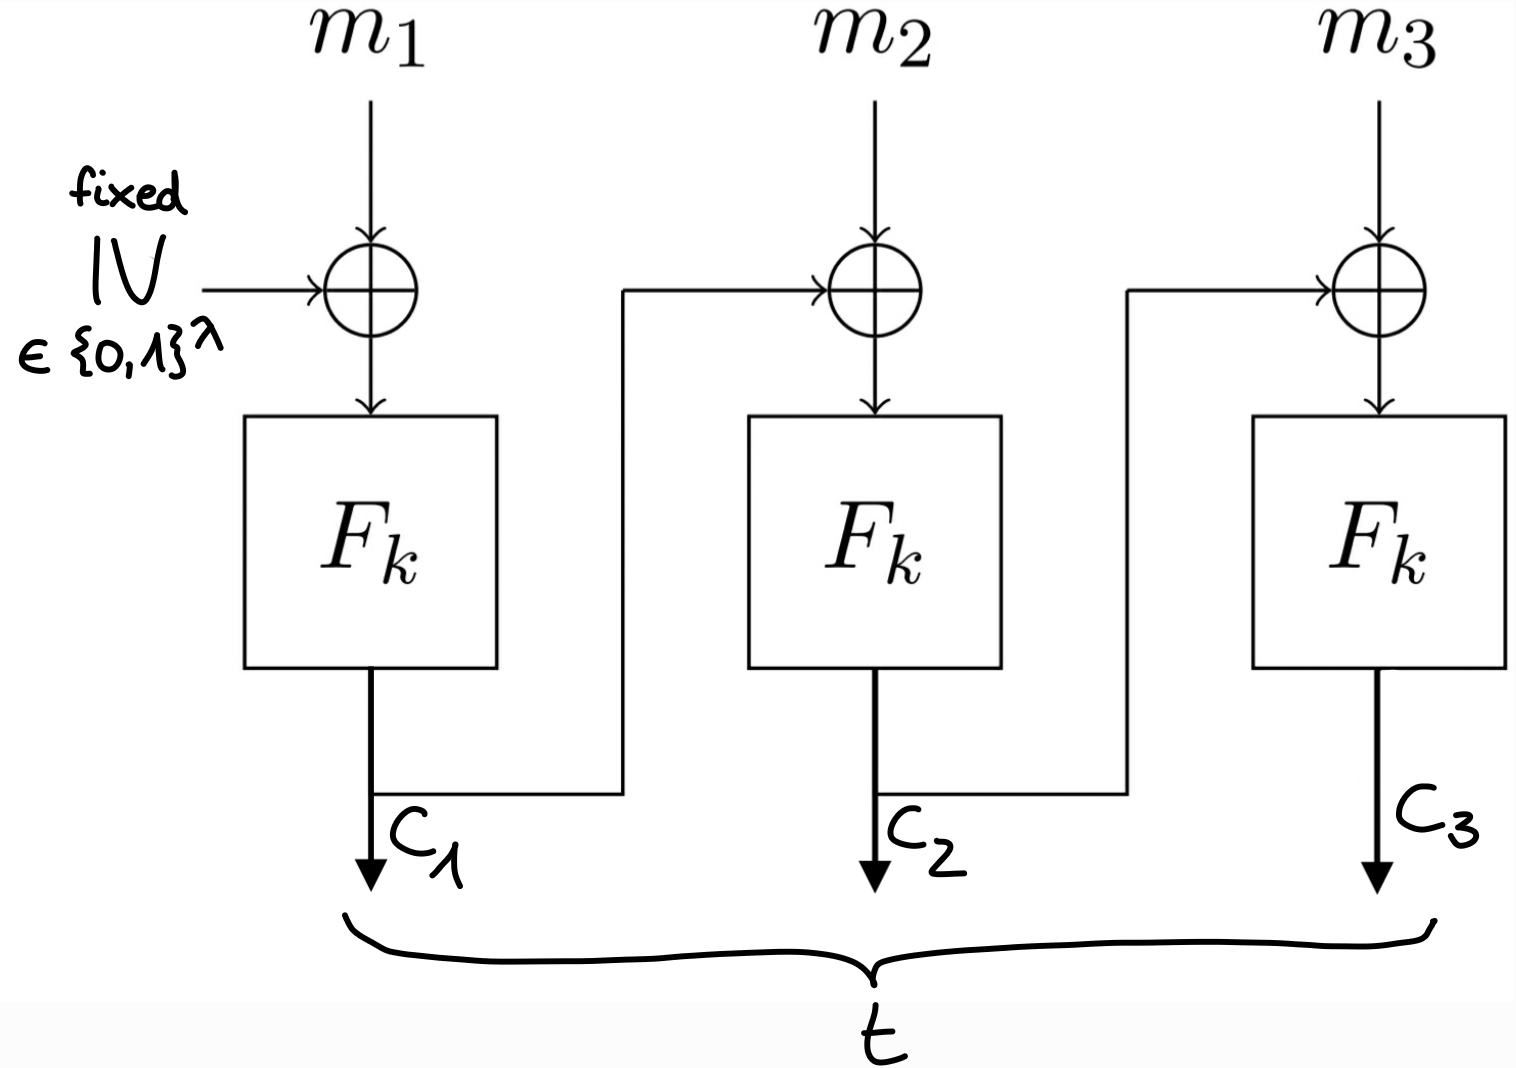
\includegraphics[width=\textwidth,height=\textheight,keepaspectratio]{ModKrypt_7-3b.jpg}
    \centering
\end{figure}

The adversary \(\mathcal{A}\) can choose the messages m of length \(\ell\)(\(\lambda\)) \(\cdot\) \(\lambda\). We set \(\ell\)(\(\lambda\)) = l. We choose \\
m\(^{1}\) = m\(_{1}^{1}\) \(\vert \vert\) ...  \(\vert \vert\)  m\(_{l}^{1}\) and\\ 
m\(^{2}\) = m\(_{1}^{2}\) \(\vert \vert\) ...  \(\vert \vert\)  m\(_{l}^{2}\) \\
with m\(_{j}^{1}\) = m\(_{j}^{2}\) =  0\(^{\lambda}\) for 2 \(\leq\) j \(\leq\) l.\\
\\
c\(_{1}^{i}\) = F\(_{k}\)(IV \(\xor\) m\(_{1}^{i}\)) with IV \(^{*}\) \(\in\) \(\{\)0,1\(\}\)\(^{\lambda}\) as a fixed vector \\
c\(_{2}^{i}\) = F\(_{k}\)(c\(_{1}^{i}\) \(\xor\) m\(_{2}^{i}\))\\
... \\
c\(_{l}^{i}\) = F\(_{k}\)( ... F\(_{k}\)(IV \(\xor\) m\(_{1}^{i}\)) ...) \\
t = (c\(_{1}^{i}\), ..., c\(_{l}^{i}\)) for i \(\in\) \(\{\)1,2\(\}\) \\
\\
To break the security of the MAC the adversary \(\mathcal{A}\) can construct the following forgery: \\
m =  m\(_{1}^{2}\) \(\vert \vert\) m\(_{2}\)´ \(\vert \vert\) m\(_{3}^{1}\) \(\vert \vert\) ...  \(\vert \vert\) m\(_{l}^{1}\) \\
with m\(_{2}\)´ = c\(_{1}^{1}\) \(\xor\) m\(_{2}^{1}\) \(\xor\) c\(_{1}^{2}\) which generates a vector that satisfies the following equation:\\
\(\Rightarrow\) c\(_{1}^{1}\) \(\xor\) m\(_{2}^{1}\) = c\(_{1}^{2}\) \(\xor\) m\(_{2}\)´  \\
This helps us construct m such that c\(_{2}^{1}\) = F\(_{k}\)(c\(_{1}^{1}\) \(\xor\) m\(_{2}^{1}\)) = F\(_{k}\)(c\(_{1}^{2}\) \(\xor\) m\(_{2}\)´) = c\(_{2}\) and c\(_{i}^{1}\) = c\(_{i}\) for i \(\in\) \(\{\)3,l\(\}\).\\
Therefore the adversary \(\mathcal{A}\) can create the valid forgery (m, t) with t = (c\(_{1}^{2}\), c\(_{2}^{1}\), ... , c\(_{l}^{1}\)) for m which has not been queried before and can break the unforgability of the Mac.

\end{itemize}
